\documentclass{article}
\usepackage{tikz}
\begin{document}
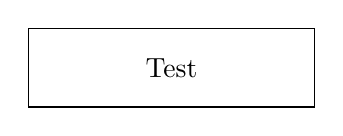
\begin{tikzpicture}
  \draw (0,0) rectangle (0.3\linewidth,1) node[pos=0.5] {Test};
\end{tikzpicture}

\begin{tikzpicture}
  \draw (0,0) rectangle (1,1) node[pos=0.5] {Test};
\end{tikzpicture}

\begin{tikzpicture}
  \draw (0,0) rectangle (1,1) node[pos=0.5] {Test};
\end{tikzpicture}

\begin{tikzpicture}
  \draw (0,0) rectangle (1,1) node[pos=0.5] {Test};
\end{tikzpicture}

\begin{tikzpicture}
  \draw (0,0) rectangle (1,1) node[pos=0.5] {Test};
\end{tikzpicture}

\begin{tikzpicture}
  \draw (0,0) rectangle (1,1) node[pos=0.5] {Test};
\end{tikzpicture}

\begin{tikzpicture}
  \draw (0,0) rectangle (1,1) node[pos=0.5] {Test};
\end{tikzpicture}

\begin{tikzpicture}
  \draw (0,0) rectangle (1,1) node[pos=0.5] {Test};
\end{tikzpicture}
\end{document}
